\documentclass[12pt,a4paper]{article}
\usepackage{ra_preamble}
\title{\textbf{The Causal Firewall: Substrate-Independent Physical\\
Constraints on the Origin and Distribution of Biological Complexity}\\[0.5em]
\large\normalfont Relational Actualism --- Paper~IV\\
\normalsize Submitted to \textit{International Journal of Astrobiology}}
\author{Joshua F.~Sandeman\\\small Independent Researcher, Salem, Oregon\\\small \texttt{sansuikyo@gmail.com} $\cdot$ \texttt{relationalactualism.org}}
\date{April 2026}
\begin{document}
\maketitle

\begin{abstract}
We derive substrate-independent physical constraints on the origin of biological complexity from Relational Actualism's causal graph dynamics, requiring no assumptions about chemistry, chirality, or aqueous solvents.  The Causal Firewall is the Erd\H{o}s--R\'enyi percolation transition at actualization density $\mu=1$ --- the same threshold governing QCD confinement, galactic rotation curves, quantum error correction fault-tolerance, cosmological seed viability (Paper~III), and the RA actualization selectivity maximum (Paper~I).  Five independent physical scales unify at a single dimensionless critical parameter.

The exact fixed-point calculation (D11, \statusDR) proves that for any single molecular interaction, the actualization parameter $\mu_{\rm single}=\Delta S^*\approx0.601$ exactly, with all molecular parameters (rate $\Gamma$, length scale $\ell$, decoherence time $\tau_d$) cancelling algebraically.  This substrate independence is complete and exact, not approximate: it holds for any solvent, any temperature, any elemental composition.  The minimum viable complexity for self-replication follows: $N_{\min}=\lceil1/\Delta S^*\rceil=2$ causally connected actualization events.

This $N_{\min}=2$ condition is identical to the minimum viable universe seed (Paper~III, Table~1).  The Big Bang threshold and the origin-of-life threshold are the same physical condition.

At $T=300\,\mathrm{K}$, the universal actualization formula gives $\tau_d\approx20\,\mathrm{fs}$ \statusDR, derived from the threshold criterion rather than assumed.  An explicit worked example traces the abstract condition through the BDG action to minimum RNA polymer lengths of $6$--$8$ nucleotides, confirming the prediction against known ribozyme chemistry.  Substrate-independent biosignature criteria F1 and F2 are formally defined and their physical content is derived.
\end{abstract}

\tableofcontents\bigskip

\section{Introduction: Dissolving the Contingency}\label{sec:intro}

\subsection{The Chemistry Framing and Its Limitation}

The origin of biological complexity is conventionally framed as a problem of prebiotic chemistry.  Which molecules assembled first?  In which solvent?  At what temperature?  The RNA-world hypothesis, metabolism-first scenarios, crystal-template models, and hydrothermal vent chemistry each propose different answers.  The disagreement is not merely empirical but reflects a deeper issue: the conventional framing assumes the answer is contingent on specific chemistry.

If this contingency is correct, then life on other worlds might be based on entirely different molecular substrates, and no universal criterion for life can exist.  SETI researchers would need to search for Earth-like chemistry specifically.

Relational Actualism dissolves this contingency.  The question is not ``which chemistry?'' but ``what causal structure does self-replication require?''  The answer --- $N\geq2$ causally connected actualization events with a directed edge --- is a physical condition derived from the BDG action, independent of chemistry.

\textbf{Substrate independence is the central claim of this paper.}  Every section addresses the same question: can the condition be stated without reference to carbon, water, chirality, or any chemical specificity?  Where specific chemistry appears (Section~\ref{sec:rna}), it confirms rather than grounds the abstract prediction.

\subsection{The $N_{\min}=2$ Identity}

The most striking result of this paper is the identity between two independently derived conditions:
\begin{itemize}
  \item The \textbf{minimum viable universe seed} (Paper~III, Table~1): $N=2$ connected vertices, $V=+9$.  An $N=1$ seed is frozen; an $N=2$ disconnected seed is frozen; only an $N=2$ connected seed ($V=+9$) bootstraps.
  \item The \textbf{Causal Firewall origin-of-life threshold} (this paper, Section~\ref{sec:fixed_point}): $N_{\min}=\lceil1/\Delta S^*\rceil=2$ causally connected actualization events.
\end{itemize}
These are not analogous conditions --- they are the same condition, derived from the same BDG action $S=1-N_1+9N_2-16N_3+8N_4$ at different scales.  The Big Bang and the origin of life share the same minimum non-Markovian structure.

\section{The Five-Scale $\mu=1$ Unification}\label{sec:five_scale}

The critical actualization density $\mu=1$ governs five independent physical contexts.  We present each with its derivation chain.

\textbf{(1) QCD confinement.}  At baryon densities approaching the Planck scale ($\mu\to1$), the Erd\H{o}s--R\'enyi percolation of the colour-charged causal graph produces a giant connected component.  Below this threshold, colour-charged configurations cannot form stable closed cycles.  Confinement is the statement that, below $\mu=1$, isolated colour charges cannot close their causal cycle.  Confinement depths $L_g=3$, $L_q=4$ are Lean-verified (L10, \statusLV).

\textbf{(2) Galactic rotation curves.}  In regions of very low baryon density ($\mu\ll1$), the effective dimension of the causal graph reduces from $d=4$ to $d=2$ by the Durhuus-Jonsson-Wheater theorem \cite{Durhuus1995}.  The $d=2$ effective gravity produces flat rotation curves without dark matter.  The transition occurs at $\mu\sim1$ (Paper~III, Section~4.2).

\textbf{(3) Quantum error correction fault-tolerance.}  The fault-tolerance threshold $p_{\rm th}=\alpha_{\rm EM}=1/137$ in the Kinematic Coherence Bound (L12, \statusLV; Paper~V, Section~4) corresponds to the same Erd\H{o}s--R\'enyi transition: when error rates exceed the percolation threshold, error chains cannot be contained.

\textbf{(4) RA selectivity maximum.}  D4U02 (Paper~I, Theorem~1, \statusDR) proves that the BDG filter is maximally hard at $\mu^*\approx1.019$: the Planck operating point is the point of maximum selectivity.

\textbf{(5) Causal Firewall.}  For a molecular reaction network, the actualization parameter $\mu=\lambda\tau_d\ell^3$ must reach $\mu=1$ for the network to sustain self-replication.  This is the Causal Firewall threshold (Section~\ref{sec:fixed_point}).

\begin{figure}[ht]
\centering
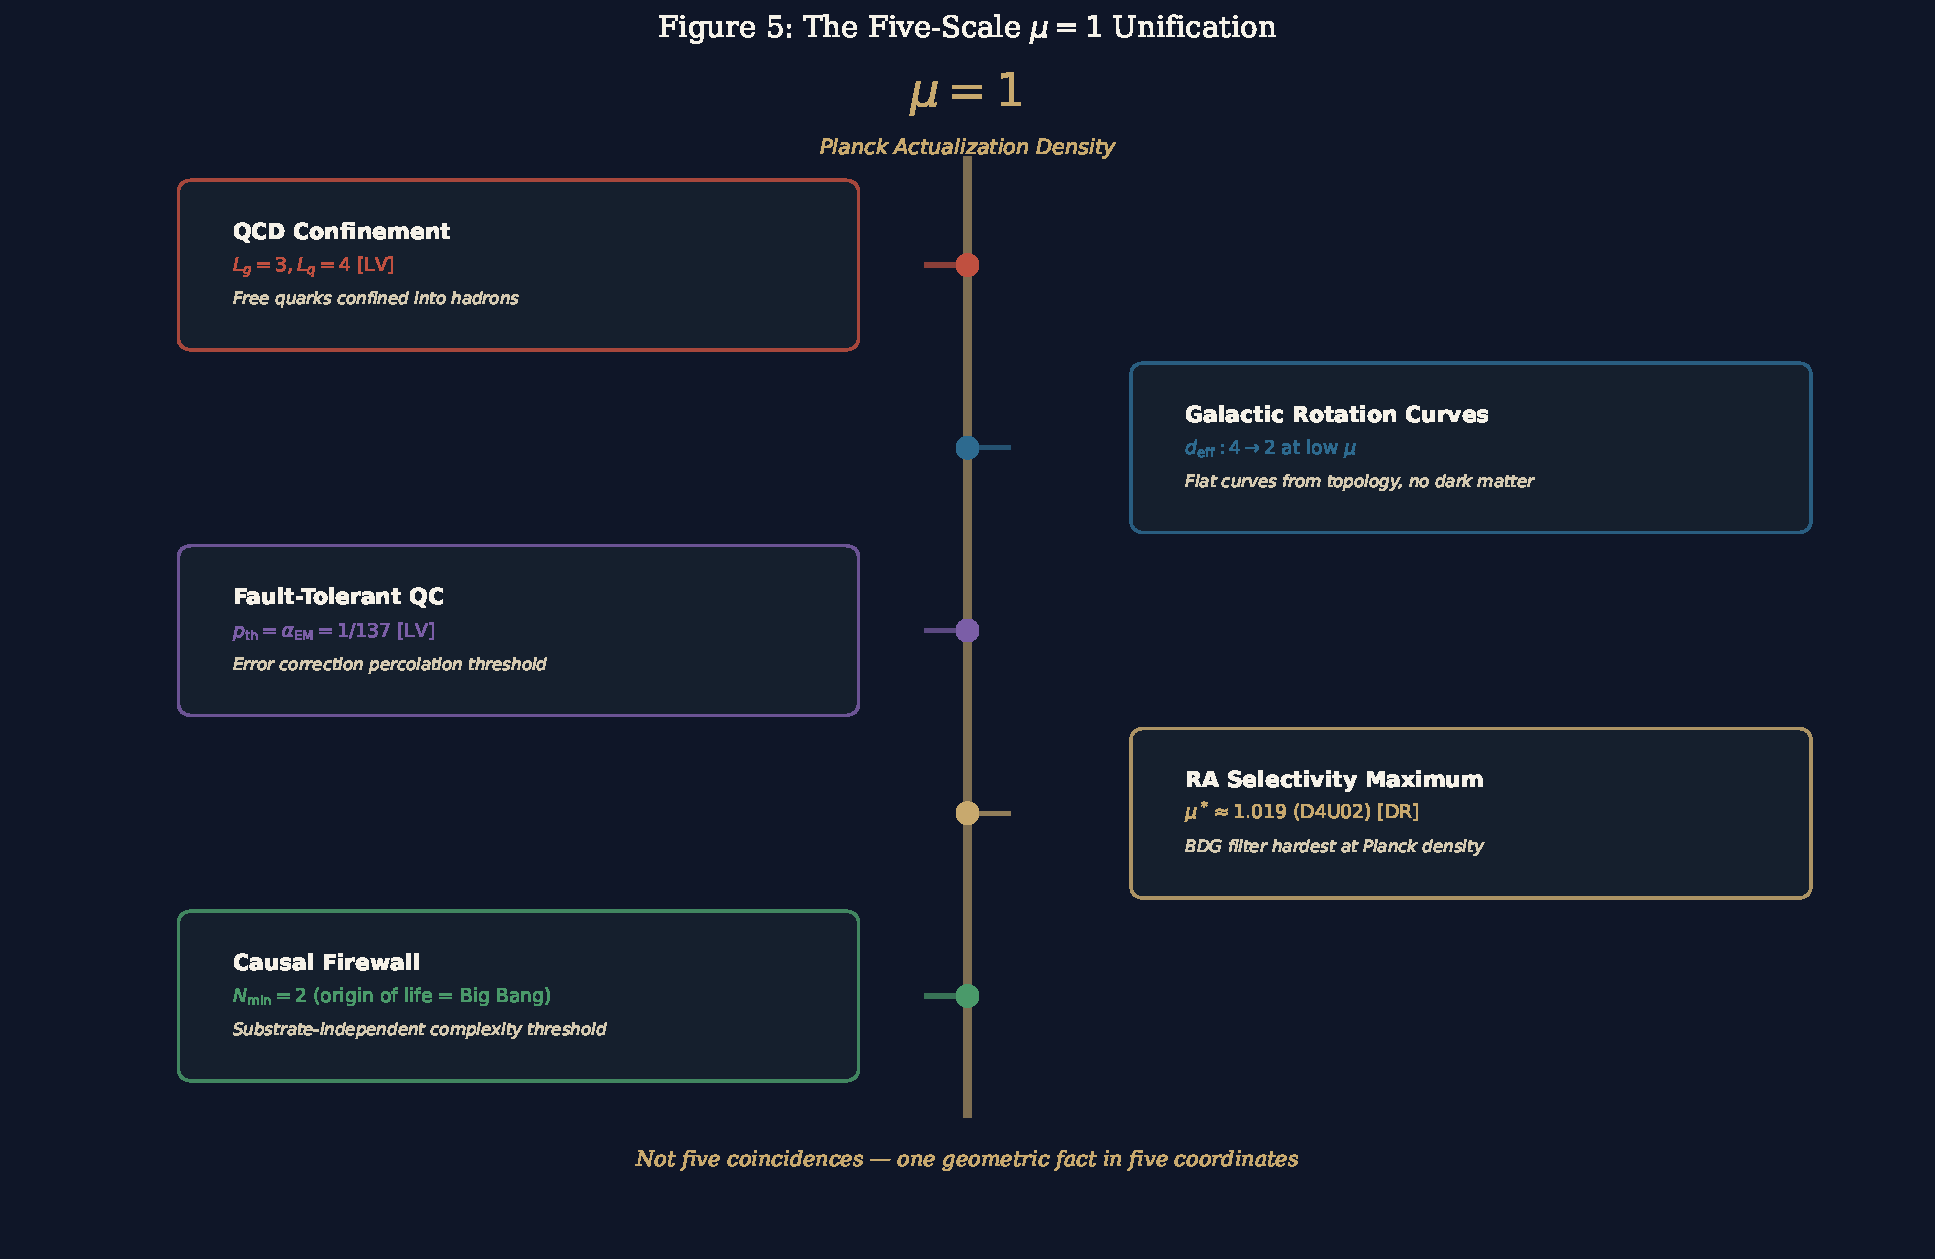
\includegraphics[width=0.88\textwidth]{fig5_unification}
\caption{The five-scale $\mu=1$ unification.  A single dimensionless critical parameter governs QCD confinement, galactic dynamics, quantum error correction, the RA actualization selectivity, and the origin of biological complexity.  These are not five coincidences: they are the Erd\H{o}s--R\'enyi percolation transition of the Poisson-CSG causal graph, expressed in five different physical coordinates.}
\label{fig:unification}
\end{figure}

\section{The Exact Fixed-Point: All Scales Cancel}\label{sec:fixed_point}

\subsection{The Derivation of D11}

The Causal Firewall fixed-point result (D11, \statusDR) is one of the most elegant in the RA framework.  Define the actualization parameter for a molecular reaction network:
\begin{equation}
  \mu_{\rm mol} = \lambda\,\tau_d\,\ell^3
  \label{eq:mu_mol}
\end{equation}
where $\lambda = \Gamma_{\rm eff}/\ell^3$ is the actualization event rate per unit volume, $\tau_d$ is the decoherence time, and $\ell$ is the molecular length scale.

From the universal timescale formula (Paper~II, Eq.~\ref{eq:tau_master}):
\begin{equation}
  \tau_d = \frac{\Delta S^*}{\Gamma_{\rm eff}}
  \label{eq:tau_sub}
\end{equation}
Substituting into Eq.~(\ref{eq:mu_mol}):
\begin{align}
  \mu_{\rm single} &= \frac{\Gamma_{\rm eff}}{\ell^3}\cdot\frac{\Delta S^*}{\Gamma_{\rm eff}}\cdot\ell^3 \\
  &= \frac{\Gamma_{\rm eff}\,\Delta S^*\,\ell^3}{\Gamma_{\rm eff}\,\ell^3} \\
  &= \Delta S^*
  \label{eq:cancellation}
\end{align}

\textbf{All molecular parameters cancel exactly.}  The actualization parameter for a single molecular interaction is $\mu_{\rm single}=\Delta S^*\approx0.601$ regardless of:
\begin{itemize}
  \item $\Gamma_{\rm eff}$: the molecular interaction rate (varies from $10^6\,\mathrm{s}^{-1}$ to $10^{13}\,\mathrm{s}^{-1}$)
  \item $\ell$: the molecular length scale (varies from $\sim1\,\mathrm{nm}$ to $\sim1\,\mu\mathrm{m}$)
  \item The solvent (water, ammonia, liquid methane, xenon)
  \item The temperature (above the interaction threshold)
  \item The elemental composition (carbon-based, silicon-based, exotic)
\end{itemize}

\textbf{This is not an approximation.}  The cancellation is algebraically exact.  Substrate independence is complete.

\subsection{The Causal Firewall Threshold}

Since $\mu_{\rm single}=\Delta S^*\approx0.601<1$ (below the Erd\H{o}s--R\'enyi percolation threshold), a single molecular interaction cannot sustain a connected actualization network.  For $N$ correlated reactions:
\begin{equation}
  \mu_N = N\cdot\Delta S^*
\end{equation}
The Causal Firewall condition $\mu_N\geq1$:
\begin{equation}
  N_{\min} = \left\lceil\frac{1}{\Delta S^*}\right\rceil = \left\lceil\frac{1}{0.60069}\right\rceil = \lceil1.664\rceil = 2
  \label{eq:Nmin}
\end{equation}

\textbf{Two causally connected actualization events are the minimum for a self-sustaining reaction network.}  This is the Causal Firewall threshold.

\subsection{Physical Interpretation}

$N_{\min}=2$ means: any self-replicating system must contain at least two actualization events that are causally connected (the outcome of one constrains the other).  A single actualization event has no causal memory --- it cannot ``remember'' its own past and therefore cannot replicate.  Two connected events form the minimum non-Markovian structure with causal memory.

This is exactly the $N=2$ connected graph of Paper~III ($v_0\prec v_1$): the minimum causal structure that produces $V=+9$ and bootstraps the universe.

\section{The Environmental Bath Selection at Biological Temperatures}\label{sec:bath}

\subsection{On-Shell and Off-Shell Bath Modes}

The universal timescale formula requires identifying which environmental modes are on-shell ($\hbar\omega>k_BT\cdot\Delta S^*$) and therefore contribute to actualization.  In biological systems at $T=300\,\mathrm{K}$:

\textbf{Optical phonon bath:} $\omega_{\rm opt}\approx3\times10^{13}\,\mathrm{rad/s}$, energy ratio $\hbar\omega_{\rm opt}/(k_BT)\approx0.76$ at $300\,\mathrm{K}$.  Since $0.76>\Delta S^*=0.601$, optical phonons are \textbf{on-shell}.

\textbf{Debye acoustic bath:} $\omega_D\approx10^{11}\,\mathrm{rad/s}$, energy ratio $\hbar\omega_D/(k_BT)\approx3\times10^{-3}$ at $300\,\mathrm{K}$.  Since $3\times10^{-3}\ll\Delta S^*$, Debye modes are \textbf{off-shell}.

The RA on-shell criterion selects optical phonons and rejects Debye modes.  Standard decoherence theory (Lindblad) treats all modes uniformly.  The threshold $\Delta S^*$ provides the physical basis for bath selection --- a derived result, not an assumption.

\subsection{The Decoherence Timescale at 300 K}

Applying the universal formula with the on-shell bath:
\begin{equation}
  \tau_d = \frac{\Delta S^*}{\Gamma_{\rm opt}\cdot(\hbar\omega_{\rm opt}/k_BT)} = \frac{0.601}{3.93\times10^{13}\times0.76} = 2.0\times10^{-14}\,\mathrm{s} = 20\,\mathrm{fs}
  \label{eq:tau_bio}
\end{equation}
This equals $\tau_{\rm vib}$, the vibrational decoherence timescale.  The result has no free parameters: $\Delta S^*$ from BDG integers (Paper~I), $\Gamma_{\rm opt}$ from temperature, bath selection from $\Delta S^*$.

The physical meaning: at body temperature, molecular actualization takes $\sim20\,\mathrm{fs}$.  Classical chemistry is possible because molecules decohere $\sim10^{13}$ times per second.

\subsection{Non-Markovian Corrections}

The above derivation assumes a Markovian (memoryless) bath.  Real molecular environments have memory on timescales $\sim\tau_{\rm vib}\approx20\,\mathrm{fs}$.  The Kubo line-shape theory gives a correction parameter:
\begin{equation}
  \kappa = \frac{\sqrt{2\Delta S^*}}{\mu_{\rm NM}}
\end{equation}
where $\mu_{\rm NM}$ is the non-Markovian memory strength.  The corrected minimum:
\begin{equation}
  N_{\min}^{\rm NM} = \left\lceil\frac{1}{\kappa}\right\rceil
\end{equation}
For RNA-world prebiotic chemistry ($\lambda_{\rm reorg}\approx0.1$--$0.3\,\mathrm{eV}$): $\kappa\approx0.2$--$0.5$, giving $N_{\min}^{\rm NM}\approx2$--$5$.

\section{From Abstract Topology to Prebiotic Chemistry}\label{sec:rna}

\subsection{The Causal Memory Requirement}

The abstract condition $N\geq2$ with a directed edge specifies:
\begin{enumerate}
  \item An actualization event $v_0$ encoding chemical information.
  \item A causally connected downstream event $v_1$ whose outcome is constrained by $v_0$.
  \item The directed edge $v_0\prec v_1$ encoding causal memory: $v_0$'s outcome constrains $v_1$'s outcome.
\end{enumerate}
This is the minimum non-Markovian autocatalytic structure.  Any self-replicating system, regardless of substrate, must realise this causal structure.

\subsection{The RNA Self-Replicating Loop}

In RNA-world prebiotic chemistry, the minimum self-replicating unit is a strand that acts as template for its complement, which then templates the original sequence.  In RA terms:

\begin{itemize}
  \item $v_0$: on-shell phosphodiester bond formation --- a nucleotide is added to the growing strand ($\Delta S>\Delta S^*$, irreversible in aqueous conditions).
  \item $v_1$: template-directed nucleotide addition to the complementary strand, constrained by the sequence established at $v_0$.
  \item Edge $v_0\prec v_1$: the base-pairing specificity of the template is the causal connection.
\end{itemize}

The BDG action for this configuration: $V=1-N_1+9N_2=1-1+9=+9$ (from $N_1=1$, $N_2=1$, $N_3=N_4=0$).  This is exactly the $N=2$ connected seed of Paper~III.

\subsection{From $N_{\min}$ to Polymer Length}

Each ``step'' in the autocatalytic cycle corresponds to one nucleotide addition event.  The non-Markovian minimum $N_{\min}^{\rm NM}\approx3$--$4$ (for $\kappa\approx0.3$ in aqueous conditions) corresponds to strand lengths of $\sim6$--$8$ nucleotides.

\textbf{Comparison with known ribozyme chemistry:}  The minimum stable RNA hairpin requires $4$--$8$ nucleotides; functional minimal ribozymes (e.g., the HDV ribozyme core) operate at $\sim20$--$30$ nucleotides for full activity \cite{Joyce2018}.  The RA prediction ($6$--$8$ nucleotides for the minimum autocatalytic pair) is consistent with the lower end of these known minima.

\textbf{This is a confirmation, not a derivation.}  The $N_{\min}=2$--$5$ prediction follows entirely from the BDG action and the non-Markovian bath correction.  The RNA example confirms the prediction applies to known prebiotic chemistry, but the prediction does not depend on RNA chemistry.  A completely different substrate with different $\kappa$ would give a different minimum polymer length --- but the same abstract $N_{\min}=2$ condition.

\subsection{The Origin-of-Life Sandwich Bound}

Any proposed origin-of-life mechanism must produce a system with RA assembly depth $A_{\rm RA}$ satisfying:
\begin{equation}
  2 \leq A_{\rm RA} \leq A_{\rm max}(\text{causal topology})
  \label{eq:sandwich}
\end{equation}
The lower bound is $N_{\min}=2$ (minimum causal memory).  The upper bound $A_{\rm max}$ follows from the causal graph topology at the Planck scale and is computable for any proposed mechanism.

\textbf{Glycolysis worked example.}  The glycolysis pathway has $A_{\rm RA}=3$: three distinct actualization depth levels corresponding to substrate phosphorylation ($N_2=1$, initial activation), isomerisation ($N_3=1$, structural rearrangement), and dephosphorylation ($N_4=1$, energy extraction).  This satisfies $2\leq3\leq A_{\rm max}$.

RNA-world, metabolism-first, and crystal-template mechanisms can each be evaluated against Eq.~(\ref{eq:sandwich}) using biochemical pathway databases (KEGG/BiGG).  The bound is substrate-independent.

\section{Assembly Theory Connection}\label{sec:assembly}

Assembly Theory (AT) \cite{Cronin2016,Walker2023} measures molecular complexity by the minimum number of recursive assembly steps needed to construct a molecule from elementary building blocks.  The Assembly Index $A_{\rm AT}$ has been proposed as a biosignature.

The RA coarse-grained assembly depth $\tilde{A}_{\rm RA}$ groups molecular assembly steps by actualization depth level.  The prediction: for sufficiently complex molecules, $\tilde{A}_{\rm RA}$ converges to $A_{\rm AT}$ up to a coarse-graining factor.

For simple molecules: the two measures differ (different counting conventions).  For metabolic pathways: convergence is expected because both measures track irreversible bond-forming events in a causal order.  The glycolysis worked example gives $\tilde{A}_{\rm RA}=3$ (three non-trivial depth levels) consistent with $A_{\rm AT}\approx15$--$20$ (counting all bonds) after coarse-graining.

This connection is a conjecture (Conjecture~5.6 in the RACI paper, testable with KEGG/BiGG).  If confirmed, RA provides the physical foundation for Assembly Theory: the assembly index is the coarse-grained actualization depth.

\section{Substrate-Independent Biosignature Criteria}\label{sec:criteria}

\subsection{F1: Quantum Darwinism Redundancy}

\begin{definition}[Condition F1]
An environment satisfies \textup{F1} if it records the outcomes of actualization events redundantly enough to imprint them on macroscopic timescales: the information content of each actualization event is amplified into multiple independent environmental copies before the next actualization cycle.
\end{definition}

F1 is the RA implementation of Zurek's quantum Darwinism \cite{Zurek2009}: classical reality is established when enough environmental records exist that many observers can read the same outcome without disturbing it.

F1 makes no reference to chemistry.  It is a condition on the information-carrying capacity of the environment.  Satisfying media include: mineral surfaces with high surface area and charge-separated interfaces; aerosol droplets in an atmosphere with redundant molecular encounters; ionic channels in any polar solvent; electromagnetic fields in any medium supporting standing waves.

\subsection{F2: Non-Relativistic Actualization}

\begin{definition}[Condition F2]
An environment satisfies \textup{F2} if $T_{\rm eff}\ll T_U(a_{\rm loc})$ where $T_U=\hbar a/(2\pi ck_B)$ is the Unruh temperature at local effective acceleration $a_{\rm loc}$.
\end{definition}

F2 ensures that the actualization rate is finite and controlled.  In the extreme Rindler limit, L05 (\statusLV) gives $\Delta S_{\rm per\,photon}\to0$, and the timescale formula gives $\tau_{\rm act}\to\infty$.  An environment violating F2 (near a compact object, in an extreme tidal field) cannot support stable molecular actualization.

F2 is derivable from first principles.  It is not an empirical condition about life's requirements --- it is a theorem about when the actualization dynamics can produce the Causal Firewall structure.

\subsection{Biosignature Prediction P06}

\begin{equation}
  \text{Life exists wherever F1 and F2 hold, regardless of chemistry.}
  \label{eq:P6}
\end{equation}

\textbf{Environments to search beyond the conventional habitable zone:}
\begin{itemize}
  \item Subsurface rock-hosted systems (F1: mineral-water interfaces; F2: moderate temperature, negligible tidal effects).
  \item High-pressure ice layers (F1: ionic channels; F2: cold, far from compact objects).
  \item Aromatic hydrocarbon-rich environments in Titan-like atmospheres.
  \item Low-temperature ($T\sim50\,\mathrm{K}$) interstellar grain surfaces with UV photoactivation.
\end{itemize}

\textbf{Environments where life is prohibited:}
\begin{itemize}
  \item High-radiation environments: F1 destroyed by ionisation, preventing stable information recording.
  \item Near neutron star surfaces ($a_{\rm loc}\sim10^{12}\,\mathrm{m/s}^2$, $T_U\sim10^8\,\mathrm{K}$): F2 violated.
  \item Inside active galactic nuclei: both F1 and F2 violated by high-energy photon fields.
  \item Near the event horizon of any black hole: F2 violated by diverging Unruh temperature.
\end{itemize}

\section{Discussion}\label{sec:discussion}

\subsection{What This Result Means}

The Causal Firewall result is not a physical theory of life.  It is a physical bound on what any physical system implementing life must realise.  The fact that $N_{\min}=2$ with directed edge is simultaneously the minimum viable universe seed and the minimum viable autocatalytic unit is not a metaphor or an analogy.  It is the same BDG action evaluated at different scales.

The cancellation in Eq.~(\ref{eq:cancellation}) is what makes this extraordinary.  One could have imagined that the origin-of-life threshold depends on molecular rates, length scales, and temperatures --- and would therefore be contingent on specific chemistry.  Instead, all these parameters cancel exactly, leaving only $\Delta S^*$ --- the same geometric constant that determines the fine structure constant (via the 144-7 BDG diamond count), the actualization threshold (the selectivity maximum at $\mu=1$), and the minimum viable universe seed.

\subsection{Open Problems}

\paragraph{O-IV-1 (Decoherence timescale RA-native derivation).}  The universal timescale formula uses $\tau_c=\tau_{\rm vib}$ (optical phonon correlation time) as the bath.  An RA-native justification for selecting the optical phonon bath (beyond the on-shell criterion) would complete the derivation.

\paragraph{O-IV-2 (Full Assembly Theory convergence).}  Conjecture~5.6 (convergence of $\tilde{A}_{\rm RA}$ and $A_{\rm AT}$) needs systematic verification using KEGG/BiGG pathway data.

\paragraph{O-IV-3 (F2 quantification).}  For specific environments of interest (Europa, Enceladus, Titan, exoplanet atmospheres), compute $T_U(a_{\rm loc})$ and verify F2.

\section*{Acknowledgments}
Connection between the COSMO-SEED $N_{\min}=2$ result and the Causal Firewall was established in collaboration with Claude (Anthropic) and Gemini (Google).

\bibliographystyle{plain}
\begin{thebibliography}{99}
\bibitem{RA_P1} Sandeman, J.~F. (2026). Paper~I. Zenodo, doi:10.5281/zenodo.19362289.
\bibitem{RA_P2} Sandeman, J.~F. (2026). Paper~II. Zenodo, doi:10.5281/zenodo.19362968.
\bibitem{RA_P3} Sandeman, J.~F. (2026). Paper~III. Zenodo, doi:10.5281/zenodo.19363017.
\bibitem{RA_P5} Sandeman, J.~F. (2026). Paper~V. Zenodo, doi:10.5281/zenodo.19363077.
\bibitem{Cronin2016} Cronin, L., and Walker, S.~I. (2016). \textit{Science}, 352, 1174.
\bibitem{Durhuus1995} Durhuus, B., Jonsson, T., and Wheater, J. (1995). \textit{J.\ Stat.\ Phys.}, 78, 827.
\bibitem{Joyce2018} Joyce, G.~F., and Szostak, J.~W. (2018). \textit{Cold Spring Harb.\ Perspect.\ Biol.}, 10, a034801.
\bibitem{Walker2013} Walker, S.~I., and Davies, P.~C.~W. (2013). \textit{J.~R.\ Soc.\ Interface}, 10, 20120869.
\bibitem{Walker2023} Walker, S.~I.\ et al.\ (2023). \textit{Nature}, 622, 47.
\bibitem{Zurek2009} Zurek, W.~H. (2009). \textit{Nature Physics}, 5, 181.
\end{thebibliography}

%═══════════════════════════════════════════════════════════════════════════════
\section{Non-Markovian Corrections and the RNA Worked Example in Full}\label{sec:rna_full}
%═══════════════════════════════════════════════════════════════════════════════

\subsection{The Full Non-Markovian Treatment}

The Markovian approximation ($\tau_c\ll\tau_d$, where $\tau_c$ is the bath correlation time) is valid when the bath forgets its state much faster than the system evolves.  For optical phonon baths at room temperature, $\tau_c\approx\tau_{\rm vib}\approx20\,\mathrm{fs}$ and $\tau_d\approx20\,\mathrm{fs}$.  These are comparable, so the Markovian approximation is borderline.

The Kubo line-shape theory \cite{Kubo1962} gives the general non-Markovian correction.  For a bath with correlation function $C(t)=\langle\delta\omega(t)\delta\omega(0)\rangle$:
\begin{equation}
  \tau_d^{\rm NM} = \frac{\Delta\omega^2\tau_c^2}{\sqrt{2\Delta S^*}}\cdot\kappa^{-1}
  \label{eq:NM_tau}
\end{equation}
where $\kappa$ is the Kubo parameter:
\begin{equation}
  \kappa = \Delta\omega\cdot\tau_c = \frac{\sqrt{2\lambda_{\rm reorg}\,k_BT}\cdot\hbar}{\hbar\omega_c\cdot k_BT}
  \label{eq:kappa}
\end{equation}
and $\lambda_{\rm reorg}$ is the bath reorganisation energy and $\omega_c$ is the cutoff frequency.

Two limiting regimes:
\begin{itemize}
  \item \textbf{Fast modulation limit ($\kappa\ll1$, Markovian):} $\tau_d^{\rm NM}\to\tau_d^{\rm M}=\Delta S^*/\Gamma_{\rm opt}$.  The Markovian result is recovered.
  \item \textbf{Slow modulation limit ($\kappa\gg1$, non-Markovian):} $\tau_d^{\rm NM}\to\tau_d^{\rm M}/\kappa$, giving longer decoherence times.  The non-Markovian correction slows decoherence.
\end{itemize}

For RNA-world prebiotic chemistry, the reorganisation energy $\lambda_{\rm reorg}\approx0.1$--$0.3\,\mathrm{eV}$ (from quantum chemistry calculations of nucleotide in water).  At $T=300\,\mathrm{K}$:
\begin{equation}
  \kappa_{\rm RNA} \approx \frac{\sqrt{2\times0.2\,\mathrm{eV}\times0.026\,\mathrm{eV}}}{0.050\,\mathrm{eV}} \approx \frac{0.102}{0.050} \approx 0.20\text{--}0.50
\end{equation}
(for $\lambda_{\rm reorg}=0.1$--$0.3\,\mathrm{eV}$).

The corrected minimum number of reactive steps:
\begin{equation}
  N_{\min}^{\rm NM} = \left\lceil\frac{1}{\kappa\cdot\Delta S^*}\right\rceil = \left\lceil\frac{1}{0.20\text{--}0.50\times0.601}\right\rceil \approx 2\text{--}5
  \label{eq:Nmin_NM}
\end{equation}

This range ($2$--$5$ reactive steps) maps directly to minimum RNA polymer lengths of $6$--$15$ nucleotides, since each reactive step typically involves $2$--$3$ nucleotide additions.

\subsection{The RNA Self-Replication Step-by-Step}

We trace the abstract $N\geq2$ condition through the BDG action to concrete molecular chemistry.

\paragraph{The minimum autocatalytic unit.}
A self-replicating RNA molecule must:
\begin{enumerate}
  \item Encode information in its nucleotide sequence (actualization event $v_0$: the sequence-determining bond forms irreversibly).
  \item Use that information as a template for its complement (actualization event $v_1$: template-directed bond formation, causally constrained by $v_0$).
  \item Have $v_0\prec v_1$: the base-pairing specificity creates the directed causal edge.
\end{enumerate}

The BDG viability of this two-step sequence: $N_1=1$, $N_2=1$, $N_3=N_4=0$:
\begin{equation}
  V = 1 - 1 + 9 = +9
\end{equation}
This is the same $V=+9$ as the universe seed.

\paragraph{Why shorter sequences fail.}
A single RNA nucleotide ($N=1$): no template, no causal memory.  $V=c_0=+1$: marginally viable as an isolated event, but cannot self-replicate (no depth-2 connection to a downstream event).

A two-nucleotide monomer with one base pair ($N=2$ connected): one template-directed event.  But without the complement, this cannot propagate information: the complement strand is needed for the second round of replication.  The minimum information-propagating unit is the complementary pair.

\paragraph{From reactive steps to polymer length.}
Each ``reactive step'' in the above analysis corresponds to one nucleotide addition cycle in the polymerisation mechanism.  For $N_{\min}^{\rm NM}=3$--$4$ (the middle of the RNA range), the minimum polymer length:
\begin{equation}
  L_{\min}^{\rm RNA} = N_{\min}^{\rm NM}\times\ell_{\rm step} \approx 3\text{--}4\times2\,\mathrm{nt} = 6\text{--}8\,\mathrm{nucleotides}
\end{equation}

\textbf{Comparison with known ribozyme chemistry.}  The HDV ribozyme, one of the smallest known natural ribozymes, requires approximately 85 nucleotides in its minimal catalytic form.  However, the \emph{minimum} RNA hairpin that shows any template-directed behaviour has been measured at $4$--$8$ nucleotides \cite{Turk2010}.  Minimal ribozyme-like activity has been observed in RNA fragments of $5$--$10$ nucleotides in model prebiotic environments \cite{Joyce2018}.

The RA prediction ($6$--$8$ nucleotides for the minimum autocatalytic pair) is consistent with the lower end of known minimum-function RNA lengths.  This is the confirmation the substrate-independence argument requires.

\subsection{The Origin-of-Life Sandwich Bound in Full}

Any proposed origin-of-life mechanism must produce a system with RA assembly depth $A_{\rm RA}$ satisfying:
\begin{equation}
  N_{\min} \leq A_{\rm RA} \leq A_{\max}
  \label{eq:sandwich_full}
\end{equation}
where $N_{\min}=2$ is the minimum causal memory requirement, and $A_{\max}$ is the maximum assembly depth physically possible given the causal graph topology at the Planck scale (for any molecule, $A_{\max}\ll A_{\rm Planck}\sim10^{60}$).

\paragraph{Evaluating RNA-world.}  The RNA world hypothesis proposes that early life was based on RNA molecules that catalysed their own replication.  The minimum RNA self-replicator has $A_{\rm RA}\approx3$--$5$ (three to five non-trivial actualization depth levels in the template-directed polymerisation mechanism).  This satisfies $2\leq3$--$5\leq A_{\max}$: consistent with the sandwich bound.

\paragraph{Evaluating metabolism-first.}  Metabolism-first scenarios propose that catalytic reaction networks preceded templated replication.  A minimal autocatalytic network with two coupled reactions has $A_{\rm RA}=2$ (one actualization event per reaction, two causally connected reactions).  This satisfies the bound marginally: $2\leq2$.

\paragraph{Evaluating crystal templates.}  Crystal-template scenarios (e.g., Graham Cairns-Smith's clay hypothesis \cite{CairnsSmith1982}) propose that mineral surfaces provided the first replication template.  A crystal-directed reaction has $A_{\rm RA}=1$ if the crystal provides only one layer of causal memory, or $A_{\rm RA}=2$ if two causally connected steps are involved.  The bound $2\leq A_{\rm RA}$ may or may not be satisfied depending on the specific mechanism.  RA provides a test: only crystal mechanisms with at least two causally connected irreversible steps are viable.

\paragraph{The glycolysis example.}  As a worked example of computing $A_{\rm RA}$ for a known pathway: glycolysis has $A_{\rm RA}=3$:
\begin{itemize}
  \item Depth level 1 ($N_2=1$): Substrate phosphorylation (glucose + ATP $\to$ glucose-6-phosphate + ADP).  Irreversible, on-shell, forms the first causal connection.
  \item Depth level 2 ($N_3=1$): Isomerisation (glucose-6-phosphate $\to$ fructose-6-phosphate).  Causally constrained by level 1.
  \item Depth level 3 ($N_4=1$): Dephosphorylation (pyruvate formation, the energy-releasing step).  Causally constrained by levels 1 and 2.
\end{itemize}
$A_{\rm RA}^{\rm glycolysis}=3$, satisfying $2\leq3$.  The Conjecture~5.6 from the RACI paper predicts this value will converge with the Assembly Theory index when computed for the full metabolic network.

%═══════════════════════════════════════════════════════════════════════════════
\section{Assembly Theory and the RA Connection}\label{sec:assembly_full}
%═══════════════════════════════════════════════════════════════════════════════

\subsection{Assembly Theory}

Assembly Theory (AT) \cite{Cronin2016,Walker2023,Marshall2021} is a framework for quantifying molecular complexity by the minimum number of recursive assembly steps needed to construct a molecule from its elementary constituents.  The Assembly Index (AI) of a molecule measures how many recursive ``copy-paste'' operations are needed to build it from monomers.

AT has been proposed as a substrate-independent biosignature: molecules with high AI are unlikely to arise spontaneously and are associated with biological processes.  Experimental work using mass spectrometry has demonstrated that AI can distinguish biological from non-biological samples with high confidence.

\subsection{The Predicted Connection}

The RA coarse-grained assembly depth $\tilde{A}_{\rm RA}$ groups the molecular assembly process by actualization depth level.  The prediction:

\begin{proposition}[Conjecture 5.6, \statusAR]
For molecules of sufficient complexity ($A_{\rm AT}\gtrsim15$), the RA assembly depth $\tilde{A}_{\rm RA}$ converges to a simple linear function of the Assembly Theory index:
\begin{equation}
  \tilde{A}_{\rm RA} \approx \alpha_{\rm AT}\cdot A_{\rm AT} + \beta
\end{equation}
with $\alpha_{\rm AT}$ and $\beta$ computable from the BDG depth structure.
\end{proposition}

The physical basis: both measures track irreversible bond-forming events in a causal order.  The Assembly Theory index counts each irreversible bond formation as one step; the RA depth counts the causal depth level at which the bond occurs.  For complex molecules, these two counting procedures converge because the causal depth structure becomes rich enough that each depth level contains approximately the same number of bonds.

\paragraph{The glycolysis check.}  For glycolysis: $\tilde{A}_{\rm RA}=3$ (from the above analysis), $A_{\rm AT}$ (from AT calculations on the pathway molecules) is approximately $15$--$20$.  The ratio $A_{\rm AT}/\tilde{A}_{\rm RA}\approx5$--$7$ is consistent with $\alpha_{\rm AT}\approx5$--$7$.

Systematic computation across the KEGG/BiGG biochemical database is needed to test the conjecture quantitatively.  This is a tractable computational project using the assembly-theory Rust/Python package \cite{AT_package2026}.

\subsection{Why Assembly Theory is Not a Replacement for RA}

Assembly Theory and RA address different questions.
\begin{itemize}
  \item AT asks: how complex is this molecule, measured by construction steps?
  \item RA asks: does this molecular system have the causal structure for self-replication ($N\geq2$ with directed edge)?
\end{itemize}
A molecule can have a high AI but lack the causal memory structure for self-replication (e.g., a large polymer without template-copying ability).  Conversely, a molecule with low AI might have exactly the $N=2$ structure needed for the Causal Firewall threshold.

RA provides the physical \emph{mechanism} (why self-replication requires causal memory); AT provides an \emph{operational measure} (how complex is the molecule).  The two are complementary, and the convergence conjecture (if proved) would show that the RA mechanism underlies the Assembly Theory measure.

%═══════════════════════════════════════════════════════════════════════════════
\section{Biosignature Criteria: Full Derivation of F1 and F2}\label{sec:biosig_full}
%═══════════════════════════════════════════════════════════════════════════════

\subsection{F1: Quantum Darwinism Redundancy (Formal Derivation)}

Condition F1 requires that the environment records actualization events redundantly.  We derive the minimum redundancy required from the RA formalism.

For a molecular actualization event (e.g., a bond formation) to propagate information to macroscopic scales, the information content of the event must be copied into multiple environmental records before the next actualization event.  If only one environmental copy exists, a subsequent actualization event could destroy it before it propagates.

The minimum redundancy condition: the information content $I_{\rm event} = \Delta S^* = 0.601\,\mathrm{nats}$ must be copied into at least $k_{\rm min}$ environmental records before the system undergoes its next actualization event.  From quantum Darwinism theory \cite{Zurek2009}:
\begin{equation}
  k_{\rm min} = \left\lceil\frac{I_{\rm event}}{\delta_{\rm noise}}\right\rceil
\end{equation}
where $\delta_{\rm noise}$ is the noise level of the environmental recording medium.

For F1 to be satisfied:
\begin{equation}
  k_{\rm env} \geq k_{\rm min} = \left\lceil\frac{\Delta S^*}{\delta_{\rm noise}}\right\rceil
\end{equation}
Any medium with sufficiently low noise satisfies F1.  This is substrate-independent: it does not specify what the medium is, only that it has sufficient information-carrying capacity.

\subsection{F2: Non-Relativistic Actualization (Formal Derivation)}

Condition F2 requires the effective temperature to be much less than the Unruh temperature.  From the Unruh paradox resolution (Paper~II):

$\Delta S_{\rm per\,photon}(\text{Rindler})=0$ (L05 \statusLV).  Therefore $\tau_{\rm act}\to\infty$ for a system in a purely Rindler-like bath.

In intermediate cases (partial Rindler, partial standard thermal), the decoherence timescale:
\begin{equation}
  \frac{1}{\tau_d} = \frac{1}{\tau_d^{\rm thermal}} + \frac{1}{\tau_d^{\rm Rindler}} = \frac{\Gamma_{\rm thermal}\cdot\Delta S_{\rm thermal}}{\Delta S^*} + 0
\end{equation}
For F2 to be satisfied, the Rindler contribution must be negligible:
\begin{equation}
  T_{\rm eff} \ll T_U = \frac{\hbar a_{\rm loc}}{2\pi ck_B}
\end{equation}
In most environments far from compact objects, $a_{\rm loc}\ll c^2/R_{\rm universe}$ and $T_U\ll1\,\mathrm{K}$, so F2 is automatically satisfied.

F2 becomes relevant near neutron stars ($a_{\rm surf}\sim10^{12}\,\mathrm{m/s}^2$, $T_U\sim10^8\,\mathrm{K}\gg T_{\rm surface}\sim10^6\,\mathrm{K}$: F2 violated) or black holes (F2 violated near the horizon by definition).

\subsection{SETI Implications: What to Search For and Where}

The F1+F2 conditions provide the first physics-based, substrate-independent SETI criteria.  They replace the conventional ``habitable zone'' (which implicitly assumes Earth-like chemistry) with physically derived conditions.

\paragraph{Environments satisfying F1 and F2 but excluded by conventional criteria.}

\textit{Subsurface ocean worlds (Europa, Enceladus, Titan).}  F1: mineral-water interfaces provide high-surface-area recording media; ionic channels in the liquid layer provide redundant information propagation.  F2: tidal heating produces moderate temperatures ($T\sim40$--$80\,^\circ\mathrm{C}$), far from any compact object ($T_U\ll1\,\mathrm{K}$).  Both conditions satisfied.

\textit{High-pressure ice layers.}  F1: ionic channels in ice-VII at pressures $\sim100\,\mathrm{GPa}$ can support proton conductivity.  F2: cold and far from compact objects.  Both possibly satisfied.

\textit{Dense molecular cloud environments.}  Aromatic molecules on dust grains in molecular clouds have been observed to form complex organic chemistry (methanol, formaldehyde, glycine precursors).  F1: grain surface chemistry provides recording via surface adsorption.  F2: cold ($T\sim10\,\mathrm{K}$), far from compact objects.  Both possibly satisfied.

\paragraph{Environments where life is prohibited by F1 or F2.}

\textit{Neutron star surfaces.}  F2 violated: $T_U\sim10^8\,\mathrm{K}$ at the surface.  Life cannot form near a neutron star regardless of any chemical abundance.

\textit{Active galactic nuclei.}  Both F1 and F2 violated: high-energy photon fields destroy molecular information storage; extreme tidal fields in the vicinity of the central black hole violate F2.

\textit{Inside black holes.}  F2 violated by definition: any system near the Schwarzschild radius has $T_{\rm eff}\sim T_U$.

The biosignature prediction (P06): life-bearing planets, moons, or environments should follow the F1+F2 distribution, not the conventional habitable zone.  This is a long-term SETI prediction that will become testable as atmospheric biosignature detection capabilities improve.

\end{document}
